\ChapterImageStar[cap:pmv]{Producto Mínimo Viable}{./images/fondo.png}\label{cap:pmv}
\mbox{}\\
\section{Código fuente del sistema}
\noindent
El código fuente del sistema, desarrollado en el lenguaje Bash, está disponible en el repositorio de GitHub \href{https://github.com/AariazP/TG-VBC.git}{\texttt{TG-VBC}} en la rama \texttt{scripted-solution}. Este repositorio contiene scripts para la automatización de tareas en la infraestructura de virtualización basada en contenedores, incluyendo la configuración de nodos, despliegue de \VM\ y configuración de Kubernetes. 
La figura~\ref{fig:estructura-proyecto} detalla la estructura del proyecto
\begin{figure}[H]
    \centering
    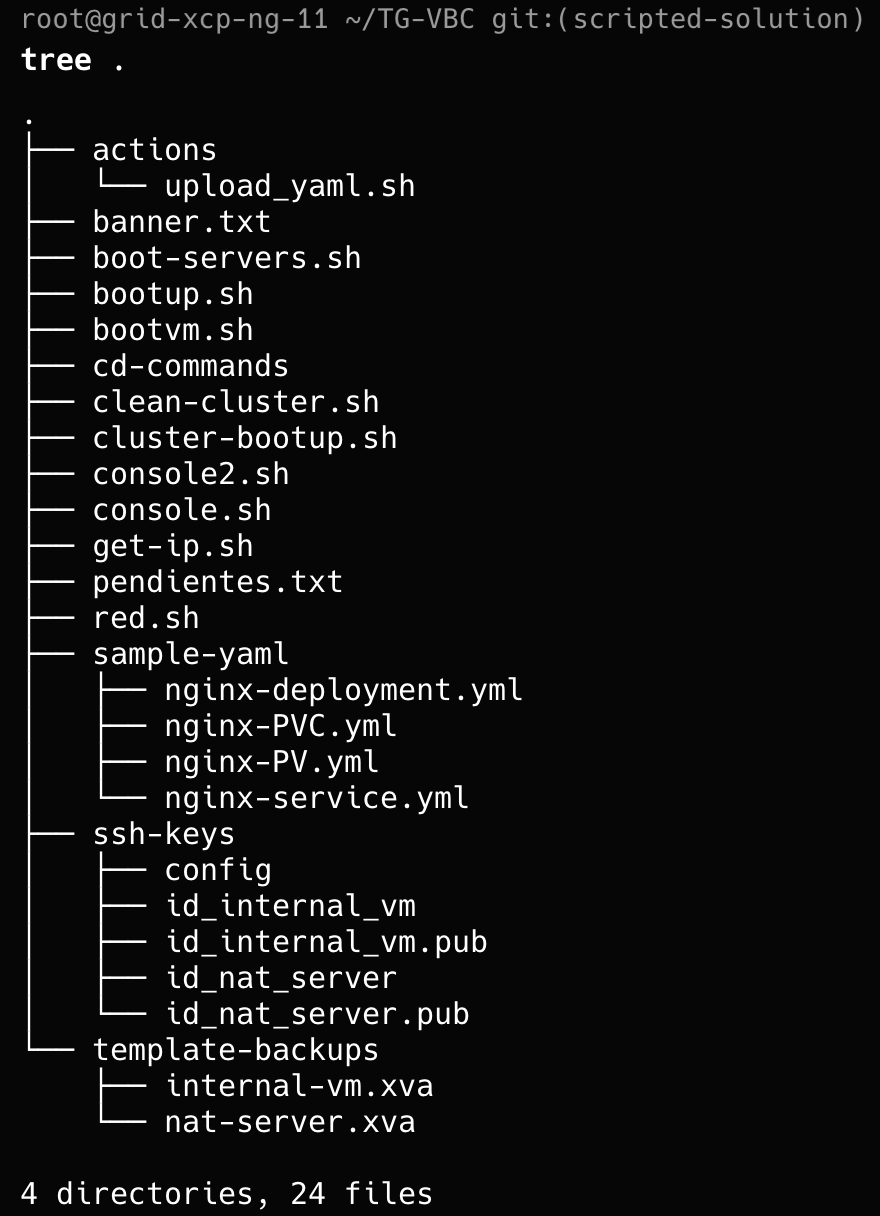
\includegraphics[scale=0.2]{tablas-images/cp6/src/tree.png}
    \caption{Estructura del proyecto}\label{fig:estructura-proyecto}
\end{figure}

\subsection{Script para obtener la IP de una VM en XCP-ng}
\noindent
El \textit{script} a continuación tiene como propósito obtener la dirección IP asociada a una \VM\ desplegada en un entorno XCP-ng, a partir de su nombre. En primer lugar, valida que el usuario haya proporcionado al menos un argumento, correspondiente al nombre de la \VM, mostrando un mensaje de uso en caso contrario. Posteriormente, contempla una excepción para la máquina denominada \textit{NAT-Master}, devolviendo directamente la IP fija 172.30.29.2. En los demás casos, el script emplea el comando xe para obtener el identificador único (UUID) de la máquina virtual y, a partir de este, extrae las direcciones \MAC\ de sus interfaces de red. Con dichas direcciones, se conecta mediante \SSH\ a la máquina \textit{NAT-Master}, utilizando una clave previamente configurada, y consulta la tabla de vecinos de red (comando ip n) para identificar la IP correspondiente a las \MAC\ recuperadas. Finalmente, devuelve la dirección IP asociada a la \VM\ solicitada. \\

\begin{minted}[frame=lines,
    fontsize=\scriptsize,
    breaklines]{bash}
#!/bin/bash

# ---------------------------------------------------------------
# Script: get-ip.sh
# Descripción:
#   Este script obtiene la dirección IP de una máquina virtual 
#   (VM) en XCP-ng a partir de su nombre.
# ---------------------------------------------------------------

# Verificación de argumentos:
# Si no se pasa al menos un argumento (nombre de la VM), se muestra 
# el uso correcto del script y se termina.
if [ $# -lt 1 ]
then
   echo "usage: get-ip <vm-name>"
   exit 0
fi

# Caso especial: 
# Si el nombre de la VM es "NAT-Master", se devuelve una IP fija 
# sin necesidad de consultar nada en XCP-ng.
if [[ "$1" == "NAT-Master" ]]
then
   echo "172.30.29.2"
   exit 0
fi

# Obtiene el UUID de la VM en XCP-ng a partir del nombre de la VM.
VM_UUID=$( xe vm-list name-label="$1" --minimal )

# Obtiene las direcciones MAC de las interfaces de red (VIFs) 
# asociadas a la VM, separadas por coma.
VM_MAC=$( xe vif-list vm-uuid="$VM_UUID" params=MAC --minimal )

# Convierte la lista separada por comas en un arreglo de MACs. 
# Se asumen máximo dos interfaces de red.
MACS=( $( echo $VM_MAC | cut -d, -f1 ) $( echo $VM_MAC | cut -d, -f2 ) )

# Redirige los errores a /dev/null para evitar mostrar mensajes 
# de advertencia de ssh u otros.
exec 2> /dev/null

# Se conecta al servidor NAT (172.30.29.2) vía SSH usando una llave 
# privada, y ejecuta el comando `ip n` (vecinos en ARP/NDP).
# Luego filtra las líneas que contengan alguna de las MACs de la VM 
# y extrae la primera columna (la IP asociada).
VM_IP=$( ssh -i ~/.ssh/id_nat_server debian@172.30.29.2 \
        "ip n | fgrep -e ${MACS[0]} -e ${MACS[1]}" | cut -d" " -f1 )

# Muestra la IP obtenida sin salto de línea adicional al final.
echo -n $VM_IP

\end{minted}


\subsection{Script de configuración de red de las VMs}
\noindent
El \textit{script} a continuación, automatiza la creación y configuración de una red virtual en un entorno XCP-ng, permitiendo la salida a Internet para las máquinas virtuales que se conecten a ella. En primer lugar, define parámetros como el nombre de la red, el rango de direcciones IP (subred), la dirección de la puerta de enlace y la interfaz de salida hacia Internet. Luego, utiliza el comando \texttt{xe network-create} para crear la red virtual sin necesidad de un \textit{bridge} preexistente y obtiene su UUID para validarla. Una vez confirmada la red, se agrega una interfaz virtual al host con una dirección \MAC\ aleatoria. Posteriormente, se asocia al bridge correspondiente la dirección IP de la puerta de enlace definida y se activa la interfaz.
\noindent
\begin{minted}[frame=lines,
    fontsize=\scriptsize,
    breaklines]{bash}
#!/bin/bash

# ---------------------------------------------------------------
# Script: red.sh
# Descripción:
#   Este script crea una red interna en XCP-ng, la configura con
#   NAT para permitir que las máquinas virtuales conectadas a ella
#   tengan salida a Internet, y habilita el reenvío de paquetes 
#   en el host.
# ---------------------------------------------------------------

# Parámetros de configuración de la red
NETWORK_NAME="vm-net-30"         # Nombre asignado a la red en XCP-ng
SUBNET="172.30.30.0/24"          # Rango de direcciones IP para la red
GATEWAY="172.30.30.1"            # Dirección IP del gateway de la red
HOST_IF_NAME="host-vif-vmnet30"  # Nombre de la interfaz virtual del host
OUT_INTERFACE="eth0"             # Interfaz del host que tiene salida a Internet

# Crear red interna sin bridge en XCP-ng
echo "Creando red virtual sin bridge..."
xe network-create name-label="$NETWORK_NAME"

# Obtener el UUID de la red recién creada
NET_UUID=$(xe network-list name-label="$NETWORK_NAME" --minimal)

# Validar que la red haya sido creada correctamente
if [ -z "$NET_UUID" ]; then
    echo "Error: no se pudo crear o encontrar la red."
    exit 1
fi

echo "Red creada con UUID: $NET_UUID"

# Crear interfaz virtual para el host en la red interna
# Esto permite que el host actúe como gateway para las VMs
HOST_UUID=$(xe host-list --minimal)

echo "Agregando interfaz virtual al host..."
xe vif-create network-uuid=$NET_UUID device=0 vm-uuid=$HOST_UUID MAC=random

# Configurar dirección IP en el bridge creado automáticamente por Xen
BRIDGE_IF=$(xe network-param-get param-name=bridge uuid=$NET_UUID)
echo "Asignando IP $GATEWAY al bridge $BRIDGE_IF..."
ip addr add $GATEWAY/24 dev $BRIDGE_IF
ip link set dev $BRIDGE_IF up

# Habilitar reenvío de paquetes IPv4 en el host
echo "Habilitando IP forwarding..."
sysctl -w net.ipv4.ip_forward=1
sed -i '/^#net.ipv4.ip_forward=1/c\net.ipv4.ip_forward=1' /etc/sysctl.conf

# Configurar reglas de NAT con iptables para salida a Internet
echo "Configurando NAT con iptables..."
iptables -t nat -A POSTROUTING -s $SUBNET -o $OUT_INTERFACE -j MASQUERADE
iptables -A FORWARD -s $SUBNET -j ACCEPT

# Guardar reglas iptables si la herramienta está disponible
if command -v netfilter-persistent &> /dev/null; then
    echo "Guardando reglas iptables con netfilter-persistent..."
    netfilter-persistent save
elif command -v iptables-save &> /dev/null; then
    echo "Puedes guardar las reglas con: sudo iptables-save > /etc/iptables/rules.v4"
fi

echo "Configuración completada. Las VMs conectadas a '$NETWORK_NAME' con IPs en $SUBNET podrán salir a Internet vía $OUT_INTERFACE."
\end{minted}

\subsection{Script de conexión SSH a una VM}
\noindent
El script a continuación, tiene como propósito facilitar la conexión remota por medio de \SSH\ a las diferentes \VM\ dentro de un entorno administrado, ofreciendo además la posibilidad de ejecutar comandos de forma directa en ellas. Su funcionamiento se puede dividir en las siguientes fases:

\begin{enumerate}
    \item \textbf{Parámetros de entrada}:  
    El script admite dos opciones principales:
    \begin{itemize}
        \item \texttt{-r}: establece que la conexión debe realizarse como el usuario \texttt{root}.
        \item \texttt{-c <comando>}: permite especificar un comando a ejecutar directamente en la máquina virtual, en lugar de iniciar una sesión interactiva.
    \end{itemize}
    Además, es obligatorio proporcionar el nombre de la VM como argumento principal.

    \item \textbf{Procesamiento de opciones}:  
    Se emplea el comando \texttt{getopts} para interpretar los parámetros recibidos. En caso de que los argumentos no cumplan con el formato esperado, se muestra un mensaje de uso correcto y el programa termina.

    \item \textbf{Resolución de la dirección IP de la VM}:  
    A través de la función auxiliar \texttt{get-ip}, el script obtiene la dirección IP asociada a la máquina virtual especificada. Los mensajes de error se redirigen a \texttt{/dev/null} para mantener una salida limpia.

    \item \textbf{Conexión mediante SSH}:  
    Existen dos escenarios:
    \begin{itemize}
        \item Si se activó la opción \texttt{-r}, la conexión se establece como el usuario \texttt{root}, utilizando una clave privada almacenada en \texttt{\~{}/.ssh/id\_internal\_vm}.
        \item En caso contrario, la conexión se realiza con el usuario por defecto, sin especificar clave adicional.
    \end{itemize}
    En ambos casos, si se definió un comando con la opción \texttt{-c}, este será ejecutado de inmediato en la máquina virtual. De lo contrario, se abrirá una sesión \SSH\ interactiva.

\end{enumerate}

\begin{minted}[frame=lines,
    fontsize=\scriptsize,
    breaklines]{bash}
#!/bin/bash

# ---------------------------------------------------------------
# Script: ssh-vm.sh
# Descripción:
#   Este script permite conectarse vía SSH a una máquina virtual 
#   en XCP-ng usando su nombre como referencia. Se puede especificar:
#   - Si la conexión debe hacerse como root.
#   - Un comando a ejecutar de forma remota en la VM.
# ---------------------------------------------------------------

# Variables iniciales
ROOT=0     # Indica si se usará el usuario root (1 = sí, 0 = no)
CMD=""     # Comando opcional a ejecutar en la VM
VM=""      # Nombre de la VM a la que se conectará

# Procesar opciones iniciales: 
#   -r  → usar root como usuario.
#   -c  → comando a ejecutar.
while getopts "rc:" opt; do
  case "$opt" in
    r) ROOT=1 ;;                # Activar conexión como root
    c) CMD="$OPTARG" ;;          # Guardar comando remoto
    *) echo "Usage: $0 [-r] <vm-name> [-c command]" >&2; exit 1 ;;
  esac
done
shift $((OPTIND - 1))            # Avanzar en la lista de argumentos

# Validar que al menos se haya pasado el nombre de la VM
if [ $# -lt 1 ]; then
  echo "Usage: $0 [-r] <vm-name> [-c command]" >&2
  exit 1
fi

# Guardar nombre de la VM y avanzar
VM="$1"
shift 1

# Reiniciar índice de opciones para procesar posibles parámetros -c después del nombre de la VM
OPTIND=1
while getopts "c:" opt; do
  case "$opt" in
    c) CMD="$OPTARG" ;;
  esac
done
shift $((OPTIND - 1))

# Obtener la dirección IP de la VM usando el script auxiliar `get-ip`
# (debe estar en el PATH del sistema).
IP=$( get-ip "$VM" 2>/dev/null )

# Conexión SSH
if [ "$ROOT" -eq 1 ]; then
  # Si se especifica conexión como root
  if [ -n "$CMD" ]; then
    # Ejecutar comando remoto como root
    ssh -i ~/.ssh/id_internal_vm root@"$IP" "$CMD" 2>/dev/null
  else
    # Abrir sesión interactiva como root
    ssh -i ~/.ssh/id_internal_vm root@"$IP" 2>/dev/null
  fi
else
  # Conexión como usuario por defecto (depende de la configuración SSH de la VM)
  if [ -n "$CMD" ]; then
    # Ejecutar comando remoto sin root
    ssh "$IP" "$CMD" 2>/dev/null
  else
    # Abrir sesión interactiva sin root
    ssh "$IP" 2>/dev/null
  fi
fi
\end{minted}

\subsection{Script de configuración inicial de una VM}
\noindent
El script \texttt{bootup.sh} fue diseñado para desplegar y configurar máquinas virtuales en XCP-ng de forma manual, en un contexto anterior a la creación de plantillas predefinidas. Aunque actualmente no se utiliza de manera habitual, se conserva como alternativa en caso de que las plantillas se pierdan o deba realizarse una instalación manual. A continuación, se detallan sus principales fases de ejecución:

\begin{enumerate}
    \item \textbf{Identificación del entorno}:  
    En primer lugar, el script lista los hosts disponibles mediante \texttt{xe host-list} y obtiene el UUID del host principal, exportándolo como variable de entorno. Posteriormente, muestra los repositorios de almacenamiento (SR) y las plantillas de sistema operativo, filtrando aquellas relacionadas con Debian.

    \item \textbf{Creación de la máquina virtual}:  
    Se define el nombre de la VM (por defecto \texttt{xeclivm} si no se pasa argumento) y se crea una nueva instancia a partir de la plantilla \texttt{Debian Bookworm 12}. A continuación, se obtiene el UUID de la VM recién creada para su uso posterior.

    \item \textbf{Gestión de medios de instalación}:  
    Se prepara un directorio local para almacenar imágenes ISO, se crea un SR de tipo ISO y se obtiene su UUID. Tras forzar un escaneo de dicho repositorio, se selecciona el archivo ISO de instalación de Debian que se utilizará para la instalación de la VM.

    \item \textbf{Configuración de almacenamiento y red}:  
    El script localiza el disco virtual asociado a la VM y lo redimensiona a 20~GiB. Asimismo, identifica el UUID de la red principal (\texttt{xenbr0}) y crea una interfaz de red para la máquina virtual.

    \item \textbf{Parámetros de hardware y arranque}:  
    Se configuran los límites de memoria de la VM (mínimos y máximos) y la política de arranque mediante BIOS. También se desactiva \textit{Secure Boot}, se fuerza el modelo tradicional de QEMU y se definen los dispositivos de arranque (disco y CD).  

    \item \textbf{Gestión de dispositivos de CD-ROM}:  
    Se expulsan posibles medios previos y se insertan las ISOs necesarias, incluyendo tanto \texttt{guest-tools.iso} como la ISO de Debian especificada. Esto asegura que la VM disponga de los medios de instalación y herramientas complementarias.

    \item \textbf{Inicio de la máquina virtual}:  
    Finalmente, la VM se arranca utilizando el UUID generado durante su creación, completando el proceso de despliegue.

\end{enumerate}

\begin{minted}[frame=lines,
    fontsize=\scriptsize,
    breaklines]{bash}
#!/bin/bash

# ---------------------------------------------------------------
# Script: bootup.sh
# Descripción:
#   Este script fue creado inicialmente para desplegar y configurar 
#   máquinas virtuales en XCP-ng de manera manual antes de contar 
#   con plantillas. Actualmente no se usa, pero se conserva como 
#   alternativa en caso de perder las plantillas predefinidas.
# ---------------------------------------------------------------

# Listar hosts disponibles
xe host-list

# Obtener UUID del host principal y exportarlo como variable de entorno
export host_uuid="$( xe host-list | grep -oP "[\d\w-]+" | grep -oP ".{20,}" | head -n 1 )"
echo "host_uuid is this : _____________ $host_uuid ______"

# Listar todos los storage repositories (SR)
xe sr-list
xe sr-list name-label="Local storage"

# Listar plantillas disponibles y filtrar Debian
xe template-list | grep Debian

# Definir nombre de la VM (por defecto "xeclivm" si no se pasa argumento)
export vm_name="${1:-xeclivm}"

# Crear nueva VM a partir de la plantilla "Debian Bookworm 12"
xe vm-install template="Debian Bookworm 12" new-name-label="${vm_name}"

# Obtener el UUID de la VM recién creada
export vm_uuid=$( xe vm-list | grep -B 1 "$vm_name" | grep -oP "[\d\w-]{20,}" )
echo "vm_uuid is this : _______________ $vm_uuid __________"

# Preparar directorio para ISO locales
mkdir -p /var/opt/xen/ISO_Store
cd /var/opt/xen/ISO_Store

# Montar un SR de tipo ISO
xe-mount-iso-sr /run/sr-mount/bedd1ebf-c12c-875d-960c-257de20dec45/

# Crear un nuevo SR para almacenar ISOs locales
xe sr-create host-uuid=$host_uuid name-label=LOCAL_ISO type=iso \
  device-config:location=/var/opt/xen/ISO_Store \
  device-config:legacy_mode=true content-type=iso

# Listar SR de tipo ISO
xe sr-list type=iso

# Obtener UUID del SR de ISOs recién creado
export sr_iso_uuid=$(xe sr-list type=iso | grep -B 1 LOCAL_ISO | head -n 1 | grep -oP "[\d\w-]+-[\w\d]+")

# Forzar escaneo del SR de ISOs
xe sr-scan uuid=$sr_iso_uuid

# Definir nombre del ISO de instalación
export cd_iso="debian-12.11.0-amd64-netinst.iso"

# Obtener UUID del disco de la VM recién creada
export vm_disk_uuid=$( xe vm-disk-list uuid=$vm_uuid | grep -B 2 "Local storage" | head -n 1 | grep -oP "[\d\w-]+-[\d\w]+" )

# Obtener UUID de la red principal (xenbr0)
export network_uuid=$( xe network-list | grep -B 3 xenbr0 | head -n 1 | grep -oP "[\d\w-]+-[\d\w]+" )

# Insertar ISO de instalación en la VM
xe vm-cd-add uuid=$vm_uuid cd-name="$cd_iso" device=1

# Configurar política de arranque de la VM
xe vm-param-set HVM-boot-policy="BIOS order" uuid=$vm_uuid

# Crear interfaz de red para la VM
xe vif-create vm-uuid=$vm_uuid network-uuid=$network_uuid device=0

# Configurar memoria de la VM (mínimo, máximo y dinámico)
xe vm-memory-limits-set dynamic-max=2048MiB dynamic-min=2048MiB \
  static-max=2048MiB static-min=512MiB uuid=$vm_uuid

# Redimensionar el disco de la VM a 20 GiB
xe vdi-resize uuid=$vm_disk_uuid disk-size=20GiB

# Configurar orden de arranque: disco y CD
xe vm-param-set uuid=$vm_uuid HVM-boot-params:order=dc

# Crear un nuevo dispositivo virtual de CD (ejemplo con UUID fijo de VDI)
xe vbd-create \
  vm-uuid=$vm_uuid \
  device=3 \
  type=CD \
  vdi-uuid=8dba583e-57df-44eb-a954-c1db24d22cc0 \
  mode=RO \
  bootable=true

# Desactivar Secure Boot y forzar emulación tradicional de QEMU
xe vm-param-set uuid=$vm_uuid platform:secureboot=false
xe vm-param-set uuid=$vm_uuid platform:device-model=qemu-traditional

# Ajustar parámetros de arranque a BIOS
xe vm-param-set uuid=$vm_uuid HVM-boot-policy="BIOS order"
xe vm-param-set uuid=$vm_uuid HVM-boot-params:firmware=bios

# Expulsar cualquier CD-ROM previo
xe vm-cd-eject uuid=$vm_uuid

# Insertar ISO de Guest Tools
xe vm-cd-insert uuid=$vm_uuid cd-name=guest-tools.iso

# Insertar ISO de Debian en la VM (usando nombre pasado como argumento $1)
xe vm-cd-insert vm=$1 cd-name=debian-12.11.0-amd64-netinst.iso

# Iniciar la VM
xe vm-start uuid=$vm_uuid
\end{minted}

\subsection{Script para desplegar y arrancar una VM desde plantilla}
\noindent
El script \texttt{bootvm} está diseñado para automatizar el despliegue y arranque de una \VM\ en un entorno XCP-ng utilizando una plantilla predefinida. Su funcionamiento se describe a continuación:

\begin{enumerate}
    \item \textbf{Validación de argumentos}:  
    El script comprueba que se haya proporcionado al menos un argumento, que corresponde al nombre deseado para la \VM. Si no se especifica ningún argumento, muestra un mensaje de uso correcto (\texttt{usage: bootvm <vm-name>}) y finaliza la ejecución.

    \item \textbf{Instalación de la máquina virtual}:  
    Se utiliza el comando \texttt{xe vm-install} para crear una nueva \VM\ a partir de una plantilla existente, identificada por su UUID (\texttt{0c838875-cb93-dfe3-8c36-a2f42183b434}). El nombre de la nueva \VM\ se asigna según el argumento proporcionado al script. El UUID de la \VM\ recién creada se almacena en la variable \texttt{VM\_UUID} para su uso posterior.

    \item \textbf{Arranque de la VM}:  
    Finalmente, el script inicia la máquina virtual mediante \texttt{xe vm-start}, utilizando el UUID almacenado previamente.

\end{enumerate}

\begin{minted}[frame=lines,
    fontsize=\scriptsize,
    breaklines]{bash}
#!/bin/bash

# ---------------------------------------------------------------
# Script: bootvm.sh
# Descripción:
#   Este script crea e inicia una máquina virtual (VM) en XCP-ng 
#   a partir de una plantilla predefinida, usando el nombre que 
#   se le pase como argumento.
# ---------------------------------------------------------------

# Validar que se haya pasado al menos un argumento (nombre de la VM)
if [ $# -lt 1 ]
then
   echo "usage: bootvm <vm-name>"
   exit 0
fi

# Crear la VM a partir de una plantilla específica (UUID de la plantilla)
# y asignarle un nombre nuevo igual al argumento pasado
VM_UUID=$(xe vm-install template=0c838875-cb93-dfe3-8c36-a2f42183b434 \
           new-name-label="$1")

# Iniciar la VM recién creada usando su UUID
xe vm-start uuid=$VM_UUID
\end{minted}

\subsection{Script para desplegar y arrancar servidores NAT}
\noindent
El script \texttt{boot-servers.sh} está diseñado para automatizar la creación e inicio de las máquinas virtuales principales responsables de la red \NAT\ en un entorno XCP-ng. Su funcionamiento puede dividirse en las siguientes fases:

\begin{enumerate}
    \item \textbf{Definición de variables y opciones}:  
    Se declara una variable \texttt{BACKUP} que indica si se debe crear un servidor \NAT\ de respaldo adicional. El script utiliza \texttt{getopts} para procesar la opción \texttt{-b}, la cual, de ser especificada, activa la creación de la máquina virtual de backup.

    \item \textbf{Creación de la máquina NAT principal}:  
    Independientemente de las opciones, el script crea la \VM\ principal denominada \texttt{NAT-Master} a partir de la plantilla \texttt{nat-server}, almacenando su UUID en la variable \texttt{MASTER\_UUID}.

    \item \textbf{Creación opcional del servidor de backup}:  
    Si se activó la opción \texttt{-b}, se crea una segunda \VM\ llamada \texttt{NAT-Backup}, también a partir de la plantilla \texttt{nat-server}, y se guarda su UUID en la variable \texttt{BACKUP\_UUID}.

    \item \textbf{Arranque de las máquinas virtuales}:  
    El script inicia la \VM\ principal mediante \texttt{xe vm-start}. Se incluye una pausa de 2 segundos para permitir que la \VM\ principal complete parcialmente su arranque antes de iniciar la \VM\ de respaldo. Si existe la \VM\ de backup, también se inicia de manera automática.

\end{enumerate}

\begin{minted}[frame=lines,
    fontsize=\scriptsize,
    breaklines]{bash}
#!/bin/bash

# ---------------------------------------------------------------
# Script: boot-servers.sh
# Descripción:
#   Este script crea e inicia las máquinas virtuales principales 
#   de red NAT en XCP-ng. Puede crear un servidor NAT principal 
#   (Master) y, opcionalmente, un servidor de respaldo (Backup) 
#   usando plantillas predefinidas.
# ---------------------------------------------------------------

# Variable que indica si se debe crear el servidor de backup
BACKUP=0

# Procesar opciones:
#   -b  → crea el servidor NAT de backup adicional
while getopts "b" opt; do
  case $opt in
    b) BACKUP=1 ;;  # Activar creación del backup
    *) echo "Usage: $0 [-w NUM_WORKERS] [-m NUM_MASTERS] [-b NAT server backup?]" >&2
       exit 1 ;;
  esac
done

# Crear el servidor NAT principal (Master) a partir de la plantilla "nat-server"
MASTER_UUID=$(xe vm-install template="nat-server" new-name-label="NAT-Master")

# Si se indicó la opción -b, crear también el servidor de backup
[[ $BACKUP > 0 ]] && BACKUP_UUID=$(xe vm-install \
     template="nat-server" new-name-label="NAT-Backup")

# Iniciar la VM principal (Master)
xe vm-start uuid=$MASTER_UUID

# Esperar 2 segundos para dar tiempo a que arranque la Master
sleep 2

# Si se creó la VM de backup, iniciarla también
[[ $BACKUP > 0 ]] && xe vm-start uuid=$BACKUP_UUID
\end{minted}

\subsection{Script para desplegar e inicializar un cluster K3s}
\noindent
El script \texttt{cluster-bootup.sh} está diseñado para automatizar la creación e inicialización de un clúster K3s sobre máquinas virtuales en XCP-ng, desplegando nodos master, worker, y opcionalmente un balanceador de carga (load balancer) y un servidor NAT de respaldo. Su funcionamiento se puede describir en varias fases:

\begin{enumerate}
    \item \textbf{Definición de variables y procesamiento de opciones}:  
    Se establecen valores por defecto para el número de nodos \texttt{master} y \texttt{worker}, así como indicadores para la creación de un servidor NAT de respaldo (\texttt{BACKUP}) y la existencia de un load balancer (\texttt{HAS\_LB}). Las opciones \texttt{-w}, \texttt{-m} y \texttt{-b} permiten al usuario modificar estas configuraciones al ejecutar el script.

    \item \textbf{Creación de servidores NAT}:  
    Se invoca el script \texttt{boot-servers} para crear el servidor NAT principal (\texttt{NAT-Master}) y, opcionalmente, un servidor de backup, según la opción \texttt{-b} proporcionada.

    \item \textbf{Creación de máquinas virtuales del clúster}:  
    Se definen los tipos de nodos (\texttt{master}, \texttt{worker} y opcionalmente \texttt{load-balancer}) y sus cantidades respectivas. A continuación, mediante un bucle se crean las VMs correspondientes utilizando el script \texttt{bootvm}.

    \item \textbf{Configuración de hostnames y archivo \texttt{/etc/hosts}}:  
    Para cada VM creada, el script espera a que la máquina obtenga su dirección IP y luego establece de manera remota el nombre de host y actualiza el archivo \texttt{/etc/hosts} mediante SSH.

    \item \textbf{Instalación de K3s}:  
    - Se identifica la IP del nodo \texttt{master1}.  
    - Si existe un load balancer, se utiliza su IP como punto de entrada TLS para la instalación del clúster K3s en \texttt{master1}.  
    - Se obtiene el token del clúster para permitir que otros nodos se unan.

    \item \textbf{Configuración del load balancer (opcional)}:  
    Si se ha creado un load balancer, se instala HAProxy, se genera una configuración básica con todos los nodos master en el backend y se aplica la configuración en el servidor, reiniciando el servicio.

    \item \textbf{Unión de nodos al clúster}:  
    Finalmente, todos los nodos master adicionales y los nodos worker se unen al clúster K3s. Se espera a que cada VM tenga IP y se ejecuta de manera remota el script de K3s especificando la URL del clúster y el token previamente obtenido.

\end{enumerate}
\begin{minted}[frame=lines,
    fontsize=\scriptsize,
    breaklines]{bash}
#!/bin/bash

# ---------------------------------------------------------------
# Script: cluster-bootup.sh
# Descripción:
#   Este script crea e inicializa un cluster K3s en XCP-ng, 
#   desplegando servidores master, workers, y opcionalmente 
#   un load balancer y un servidor NAT de backup. Configura 
#   hostnames, IPs, HAProxy (si hay load balancer) y une 
#   todos los nodos al cluster.
# ---------------------------------------------------------------

# Valores por defecto
NUM_WORKERS=2
NUM_MASTERS=1
BACKUP=0
HAS_LB=0

# Procesar opciones:
# -w NUM_WORKERS  → Número de nodos worker
# -m NUM_MASTERS  → Número de nodos master
# -b              → Crear NAT server backup
while getopts "w:m:b" opt; do
  case $opt in
    w) NUM_WORKERS=$OPTARG ;;
    m) NUM_MASTERS=$OPTARG ;;
    b) BACKUP=1 ;;
    *) echo "Usage: $0 [-w NUM_WORKERS] [-m NUM_MASTERS] [-b NAT server backup?]" >&2
       exit 1 ;;
  esac
done

# Si hay más de un master, se necesitará un load balancer
[[ $NUM_MASTERS > 1 ]] && HAS_LB=1 

# Crear servidores NAT (Master y opcionalmente Backup)
[[ $BACKUP > 0 ]] &&  boot-servers -b ||  boot-servers 

# Esperar 3 segundos para que arranquen
sleep 3

# Definir nombres y cantidad de nodos a crear
NAMES=( master worker )
VALUES=( $NUM_MASTERS $NUM_WORKERS )

# Si hay load balancer, agregarlo al arreglo
if [[ $HAS_LB > 0 ]]; then
    NAMES=( load-balancer master worker )
    VALUES=( 1 $NUM_MASTERS $NUM_WORKERS )
fi

# Crear VMs según tipo y cantidad
for idx in $( seq 0 ${#NAMES[@]} | head -n -1 ); do
    name=${NAMES[$idx]}
    value=${VALUES[$idx]} 

    # Crear cada VM del tipo correspondiente
    for i in $( seq 1 $value ); do
        bootvm $name$i
    done

    sleep 2

    # Configurar hostname y /etc/hosts en cada VM
    for i in $( seq 1 $value ); do
        echo "=== setting up $name$i hostname ==="
        
        # Esperar a que la VM tenga IP
        while [ -z $VM_IP ]; do 
            VM_IP=$( get-ip $name$i )
            sleep 1
        done

        # Configurar hostname remoto
        ssh -i ~/.ssh/id_internal_vm root@$VM_IP \
            "hostnamectl set-hostname $name$i; hostname; \
             echo '127.0.0.1 $name$i' >> /etc/hosts"

        VM_IP=""
    done
done

# Obtener IP del master1
MASTER_IP=$( get-ip master1 )

# Obtener IP del load balancer si existe
[ $HAS_LB -gt 0 ] && LB_IP=$( get-ip load-balancer1 )

# Instalar K3s en master1
if [ $HAS_LB -gt 0 ]; then
    ssh -i ~/.ssh/id_internal_vm root@$MASTER_IP \
        "curl -sfL https://get.k3s.io | sh -s - server --cluster-init --tls-san ${LB_IP}"
else
    ssh -i ~/.ssh/id_internal_vm root@$MASTER_IP \
        "curl -sfL https://get.k3s.io | sh -"
fi

# Obtener token de cluster K3s para unir nodos
while [ -z $TOKEN ]; do
    TOKEN=$( ssh -i ~/.ssh/id_internal_vm root@$MASTER_IP \
             "sudo cat /var/lib/rancher/k3s/server/node-token" )
done

# Configurar HAProxy si hay load balancer
if [[ $HAS_LB > 0 ]]; then

    # Instalar HAProxy
    ssh -i ~/.ssh/id_internal_vm root@$LB_IP "apt install haproxy -y"

    # Configuración básica de HAProxy
    config="frontend k3s-api
        bind *:6443
        default_backend k3s-masters

    backend k3s-masters
        balance roundrobin
    "

    # Agregar cada master al backend de HAProxy
    for i in $( seq 1 $NUM_MASTERS ); do
        ip=$( get-ip master$i )
        config+="    server master${i} ${ip}:6443 check
"
    done

    # Mostrar configuración
    echo "_____________________"
    echo "$config"
    echo "_____________________"

    # Subir configuración al LB y reiniciar servicio
    ssh -i ~/.ssh/id_internal_vm root@$LB_IP \
        "cat > /etc/haproxy/haproxy.cfg" <<< "$config"
    ssh -i ~/.ssh/id_internal_vm root@$LB_IP "sudo systemctl restart haproxy"

fi

# Arreglos de nombres, cantidad y modos para unir nodos
NAMES=( master worker )
VALUES=( $NUM_MASTERS $NUM_WORKERS )
MODES=( "-s - server" "-" )

# Determinar IP a la que los nodos se unirán
JOIN_IP=${LB_IP}
[ $HAS_LB -eq 0 ] && JOIN_IP=$MASTER_IP

# Unir nodos al cluster K3s
for idx in {0..1}; do
    name=${NAMES[$idx]}
    value=${VALUES[$idx]}
    mode=${MODES[$idx]}

    for i in $( seq 1 $value ); do
        # Saltar master1 que ya está inicializado
        [[ ${name}${i} == "master1" ]] && continue

        echo "=== joining host $name$i to cluster ==="

        # Esperar a que la VM tenga IP
        while [ -z $VM_IP ]; do 
            VM_IP=$( get-ip $name$i )
            sleep 1
        done

        # Ejecutar script K3s para unir nodo al cluster
        ssh -i ~/.ssh/id_internal_vm root@$VM_IP \
            "curl -sfL https://get.k3s.io | K3S_URL=https://${JOIN_IP}:6443 K3S_TOKEN=${TOKEN} sh ${mode}"

        VM_IP=""
    done
done
\end{minted}

\subsection{Script para limpiar el clúster K3s y eliminar VMs}
\noindent
El script \texttt{clean-cluster.sh} está diseñado para eliminar de manera segura todas las máquinas virtuales (VMs) asociadas a un clúster en XCP-ng, excluyendo los dominios del sistema. Puede ejecutarse de forma interactiva o automática mediante una opción de confirmación. Su funcionamiento se describe a continuación:

\begin{enumerate}
    \item \textbf{Definición de variables y procesamiento de opciones}:  
    Se declara la variable \texttt{ASSUME\_YES}, que indica si la operación de borrado debe realizarse automáticamente sin solicitar confirmación al usuario.  
    La opción \texttt{-y} activa este modo automático, lo que permite ejecutar el script de manera no interactiva.

    \item \textbf{Confirmación interactiva}:  
    Si no se ha especificado la opción \texttt{-y}, el script solicita al usuario confirmar la operación mediante un mensaje. Si la respuesta no coincide con alguna forma de \texttt{sí}, el script termina sin realizar cambios.

    \item \textbf{Obtención de las máquinas virtuales a eliminar}:  
    Se genera una lista de VMs mediante \texttt{xe vm-list}, filtrando únicamente los nombres de VM y excluyendo dominios del sistema (por ejemplo, aquellos que contienen la palabra \texttt{domain}).  

    \item \textbf{Iteración y eliminación de cada VM}:  
    Para cada VM encontrada:
    \begin{itemize}
        \item Se obtiene su UUID mediante \texttt{xe vm-list} para poder referenciarla de manera única.
        \item La VM se apaga de forma forzada en segundo plano mediante \texttt{xe vm-shutdown} y se espera a que el proceso finalice.
        \item Finalmente, la VM se elimina permanentemente del sistema mediante \texttt{xe vm-destroy}.
    \end{itemize}
\end{enumerate}
\begin{minted}[frame=lines,
    fontsize=\scriptsize,
    breaklines]{bash}
#!/bin/bash

# ---------------------------------------------------------------
# Script: clean-cluster.sh
# Descripción:
#   Este script elimina todas las máquinas virtuales (VMs) de un 
#   cluster en XCP-ng, excluyendo dominios del sistema. Puede 
#   ejecutarse de manera interactiva o automática usando la opción -y.
# ---------------------------------------------------------------

# Variable que indica si se debe asumir "sí" automáticamente
ASSUME_YES=false

# ---------------------------------------------------------------
# Procesar opción:
#   -y  → Asumir "sí" automáticamente para borrar las VMs
# ---------------------------------------------------------------
while getopts "y" opt; do
  case $opt in
    y)
      ASSUME_YES=true  # Activar borrado automático
      ;;
    *)
      echo "Usage: $0 [-y]"
      exit 1
      ;;
  esac
done

# Si no se asumió "sí", pedir confirmación al usuario
if [ "$ASSUME_YES" = false ]; then
  read -p "Are you really sure you want to clean cluster. (y/N): " resp
  [[ ! $resp =~ (y|Y|yes|Yes|YES) ]] && exit 0
fi

# Obtener lista de VMs a eliminar, excluyendo dominios del sistema
vms=$(xe vm-list | grep name-label | grep -v "domain" | grep -oP "(?<=: ).+")

# Iterar sobre cada VM encontrada
for vm in $vms; do
  # Obtener UUID de la VM
  UUID=$(xe vm-list name-label="$vm" --minimal | tr ',' ' ')
  
  # Apagar la VM de forma forzada en segundo plano
  xe vm-shutdown uuid=$UUID force=true &
  wait $!  # Esperar a que termine el apagado
  
  # Eliminar la VM del sistema
  xe vm-destroy uuid=$UUID
done
\end{minted}
